\documentclass[tikz,border=10pt]{standalone}
\usepackage{amsmath}
\usepackage{tikz}
\usetikzlibrary{arrows.meta, positioning, shapes.geometric}

\begin{document}
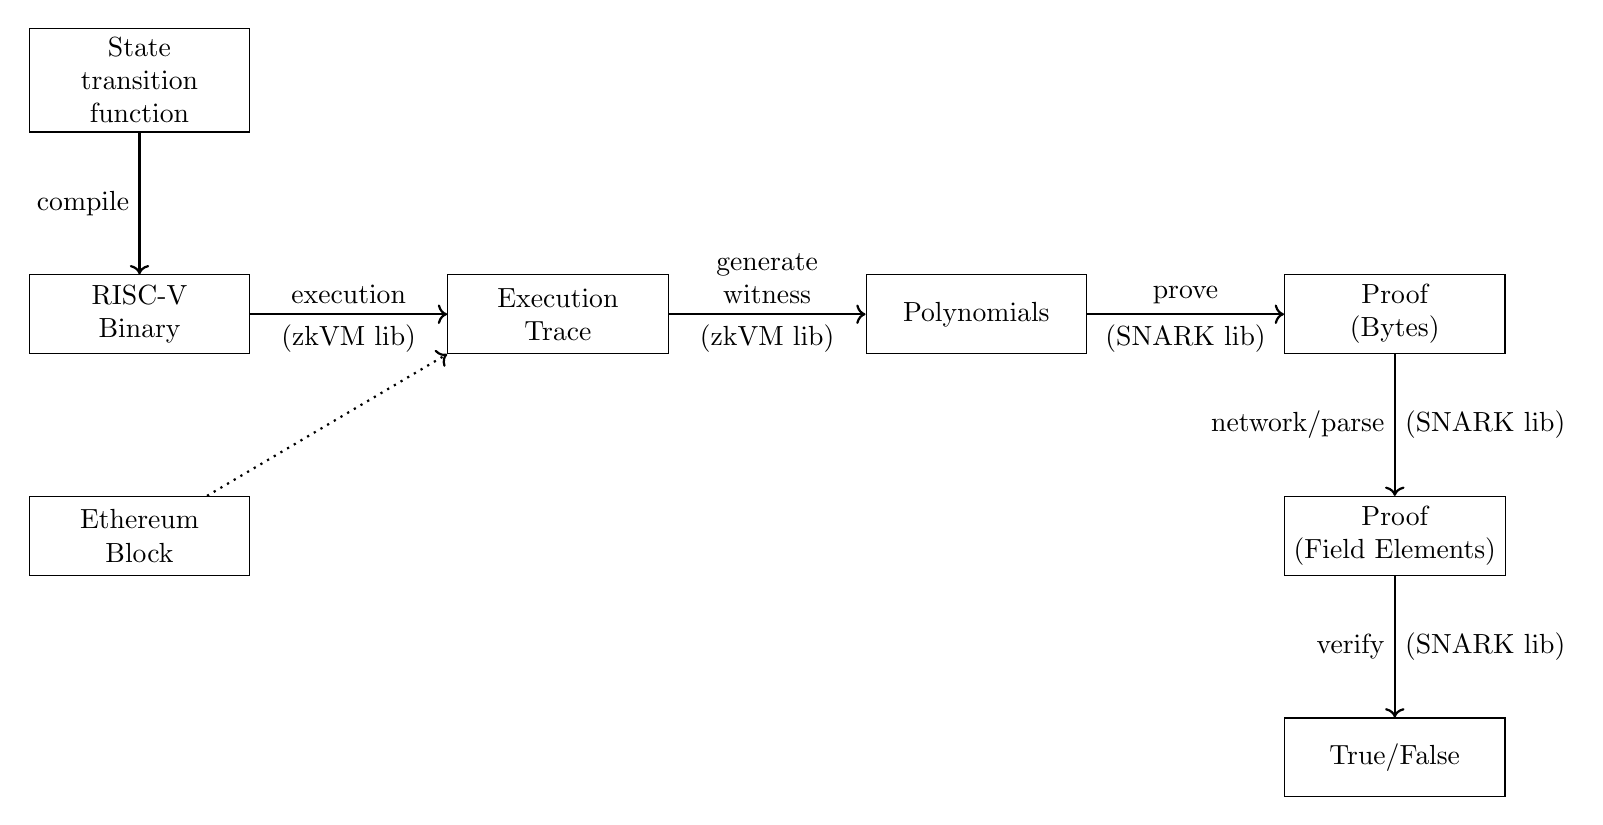
\begin{tikzpicture}[
  node distance=1.5cm and 2.5cm,
  box/.style={draw, rectangle, minimum width=2.8cm, minimum height=1cm},
  arrow/.style={->, thick},
  dottedarrow/.style={->, thick, dotted},
  every label/.style={font=\small}
]

% Nodes
\node[box, align=center] (rust) {State \\ transition \\ function};
\node[box, align=center, below=of rust, yshift=-0.3cm] (asm) {RISC-V \\ Binary};
\node[box, align=center, below=of asm, yshift=-0.3cm] (inputs) {Ethereum \\ Block};
\node[box, align=center, right=of asm] (trace) {Execution \\ Trace};
\node[box, align=center, right=of trace] (poly) {Polynomials};
  \node[box, align=center, right=of poly] (bytes) {Proof \\ (Bytes)};
  \node[box, align=center, below=of bytes, yshift=-0.3cm] (fields) {Proof \\ (Field Elements)};
\node[box, align=center, below=of fields, yshift=-0.3cm] (verdict) {True/False};

% Arrows

% Dotted vertical arrow from Inputs to Trace
\draw[dottedarrow] (inputs) -- 
  node[midway, left] {} 
  node[midway, right] {} 
  (trace.south west);

% Vertical with split labels (Code → Binary)
\draw[arrow] (rust) -- 
  node[midway, left] {compile}
  % node[midway, right] {(rustc; LLVM)} 
  (asm);

% Horizontal with stacked labels
\draw[arrow] (asm) -- 
  node[midway, above] {execution}
  node[midway, below] {(zkVM lib)} 
  (trace);

\draw[arrow] (trace) -- 
  node[midway, align=center, above] {generate \\ witness}
  node[midway, below] {(zkVM lib)} 
  (poly);

\draw[arrow] (poly) -- 
  node[midway, above] {prove}
  node[midway, below] {(SNARK lib)} 
  (bytes);

% Vertical with split labels
\draw[arrow] (bytes) -- 
  node[midway, left] {network/parse}
  node[midway, right] {(SNARK lib)} 
  (fields);

\draw[arrow] (fields) -- 
  node[midway, left] {verify}
  node[midway, right] {(SNARK lib)} 
  (verdict);
u
\end{tikzpicture}
\end{document}

